%%%%%%%%%%%%%%%%%%%%%%%%%%%%%%%%%%%%%%%%%%%%%%%%%%%%%%%%%%%%%  
%
% Sprawozdanie MOW
% TEMAT PROJEKTU: 
% AUTOR: 	Krzysztof Belewicz
%			Paweł Pieńczuk
% 23.01.2020
%
%%%%%%%%%%%%%%%%%%%%%%%%%%%%%%%%%%%%%%%%%%%%%%%%%%%%%%%%%%%%%

\documentclass[a4paper,11pt,twoside]{mwrep}  %bylo report
\usepackage[utf8]{inputenc} %ISO-8859-2 
\usepackage[UKenglish,polish]{babel} 
\usepackage[T1]{fontenc} 
\usepackage{mathptmx}
\usepackage[scaled=.90]{helvet}
\usepackage{courier}
\usepackage{gensymb} %\degree
%\usepackage[pdftex]{graphicx} 
%\usepackage{pdfpages} 
%\usepackage{wrapfig}
%\usepackage{hyperref} 
%\usepackage{gensymb}
% tablice
%\usepackage{ctable}
%\usepackage{threeparttablex}
%\usepackage{booktabs}
% grafiki
\usepackage{graphicx}
\usepackage{subfig}
\usepackage{float}
%% matematyka i greckie literki w jednostkach
\usepackage{amsmath}
\usepackage{textgreek}
%% wstawki pdf
%\usepackage{pdfpages}
% wstawki z kodem 
\usepackage{listings}
\usepackage{color}
\usepackage{url}
% Linki
\makeatletter
\g@addto@macro{\UrlBreaks}{\UrlOrds}
\expandafter\def\expandafter\UrlBreaks\expandafter{\UrlBreaks%  save the current one
  \do\a\do\b\do\c\do\d\do\e\do\f\do\g\do\h\do\i\do\j%
  \do\k\do\l\do\m\do\n\do\o\do\p\do\q\do\r\do\s\do\t%
  \do\u\do\v\do\w\do\x\do\y\do\z\do\A\do\B\do\C\do\D%
  \do\E\do\F\do\G\do\H\do\I\do\J\do\K\do\L\do\M\do\N%
  \do\O\do\P\do\Q\do\R\do\S\do\T\do\U\do\V\do\W\do\X%
  \do\Y\do\Z}
  
%\usepackage[paper=A4]{typearea}
%marginesy 
\usepackage[ bindingoffset = 0cm, hmargin = 2cm, vmargin = 2cm]{geometry} 
%interlinia 
\linespread{1} 

\widowpenalty=10000 % ostatni wierszrkapitu nie zostanie przeniesiony na następną stronę 
\clubpenalty=10000 % pierwszy wiersz akapitu nie będzie kończył strony (nie używam tego ustawienia)
\hbadness= 1450 %% zmniejsza liczę wyświetlanych ostrzeżeń (można zwiększyć, ale bez przesady)
\hfuzz = 0pt %% tekst może sterczeć ma marginesie na 1,5pt (ok. 0,5mm)

\clubpenalty=10000 %nie pozostawia sierot
\brokenpenalty=10000 %nie dzieli stron je»eli podziaª wyrazu
\sloppy %zakaz wydªu»ania lini

%wcięcia 
\setlength{\parindent}{1cm} 
\setcounter{secnumdepth}{2} %only sections and subsections are numbered 
\setcounter{tocdepth}{2} %table of contents shows up to three levels 

%\newcommand\tab[1][1cm]{\hspace*{#1}}

\begin{document} 



%%%%%%%%%%%%%%%%%%%%%%%%%%%%%%%%%%%%%%%
%			STRONA TYTUŁOWA
%%%%%%%%%%%%%%%%%%%%%%%%%%%%%%%%%%%%%%%

\begin{titlepage} 
{\begingroup
\centering 

\vspace*{15\baselineskip} 

{\Huge Metody Odkrywania Wiedzy}
\vspace*{1\baselineskip}

{\huge Dokumentacja końcowa projektu}

\vspace*{3\baselineskip}
{\LARGE „Predykcja zużycia energii na podstawie danych czujnikowych”}
\\[\baselineskip]

\vspace*{20\baselineskip} 
{\Large 
Krzysztof Belewicz\\
Paweł Pieńczuk\par} 

\vspace*{1\baselineskip}
\today

\endgroup\clearpage}
\end{titlepage} 

%%%%%%%%%%%%%%%%%%%%%%%%%%%%%%%%%%%%%%%%%%%%%%%%%%%%%%%%%%%%%   
% Sprawko właściwe
%%%%%%%%%%%%%%%%%%%%%%%%%%%%%%%%%%%%%%%%%%%%%%%%%%%%%%%%%%%%%

%TODO nazwy chapterów ukradzione z elka.mine
%TODO ciężkie wzorowanie w tym co napisane/ będzie napisane
\large %trochę cheat na objętość

\begingroup
\let\clearpage\relax
\chapter{Opis projektu} %Interpretacja tematu

Celem projektu było wyznaczenie całkowitego zużycia energii dla zadanej chwili czasu, tzn. sumy poborów sprzętów AGD (kolumna \textit{Appliances}) i oświetlenia (kolumna \textit{lights}). 
Zbiór danych został pozyskany z archiwum dostępnego na stronie: 
{\url{https://archive.ics.uci.edu/ml/datasets/Appliances+energy+prediction}}. Pojęciem docelowym jest wartość całkowitej pobieranej mocy przez gospodarstwo domowe. W ramach projektu zdecydowano się na oddzielne wykonania zadania regresji dla celu \textit{Appliances} i celu \textit{lights}, ze względu na hipotezę, że modele je wyznaczające mogą mieć inne właściwości.
\par
Dokonano selekcji atrybutów za pomocą trzech algorytmów opisanych w rozdziale \ref{chap:selekcja}. Przeprowadzono procedurę oceny algorytmów liniowej regresji, drzew regresji oraz kawałkami liniowej regresji. 

\endgroup

\begingroup
\let\clearpage\relax
\chapter{Opis danych}

\section{Charakterystyka danych}

Dane wykorzystywane do eksperymentów zostały zebrane za pomocą sieci czujników w niewielkim domu w czasie 4.5 miesiąca. 
Składają się z:
\begin{itemize}
\item[$\bullet$] daty i godziny pomiaru,
\item[$\bullet$] poboru energii sprzętów domowych [$Wh$],
\item[$\bullet$] poboru energii oświetlenia [$Wh$],
\item[$\bullet$] pomiarów temperatury i wilgotności dla 8 różnych pomieszczeń ([\degree $C$], [$\%$]),
\item[$\bullet$] pomiarów temperatury i wilgotności dla zewnętrznej, północnej strony budynku ([\degree $C$], [$\%$]),
\item[$\bullet$] danych z pobliskiej stacji pogodowej:
	\begin{itemize}
	\item[$\circ$] temperatura powietrza [\degree $C$],
	\item[$\circ$] temperatura punktu rosy [\degree $C$],
	\item[$\circ$] ciśnienie atmosferyczne [$mm~Hg$],
	\item[$\circ$] wilgotność [$\%$],
	\item[$\circ$] prędkość wiatru [$m/s$],
	\item[$\circ$] widoczność [$km$].
	\end{itemize}
\end{itemize}

\section{Przygotowanie danych}
Każdy pomiar został uśredniony z 3 próbek wykonanych w równych odstępach co ok. 3,3 min. W ramach przygotowania danych, data i godzina pomiaru zostały rozdzielone na cztery oddzielne kolumny, zawierające miesiąc, dzień, godzinę i minutę pomiaru.
\endgroup


%\pagebreak
\clearpage

%\begingroup
%\let\clearpage\relax
%\chapter{Opis algorytmów}
%
%
%TODO - ten chapter jest imo zawarty w 'konstrukcji i ocenie modeli'\\
%ergo można usunąć, grafikę przenieść tam.\\
%(chapter jest tutaj bo skopiowałem sprawko wstępne)\\
%(grafika nie wiem czemu tutaj jest, tak wyszło)\\
%
%%\begin{figure}[H]%
%%    \centering
%%    \subfloat{{
%%    	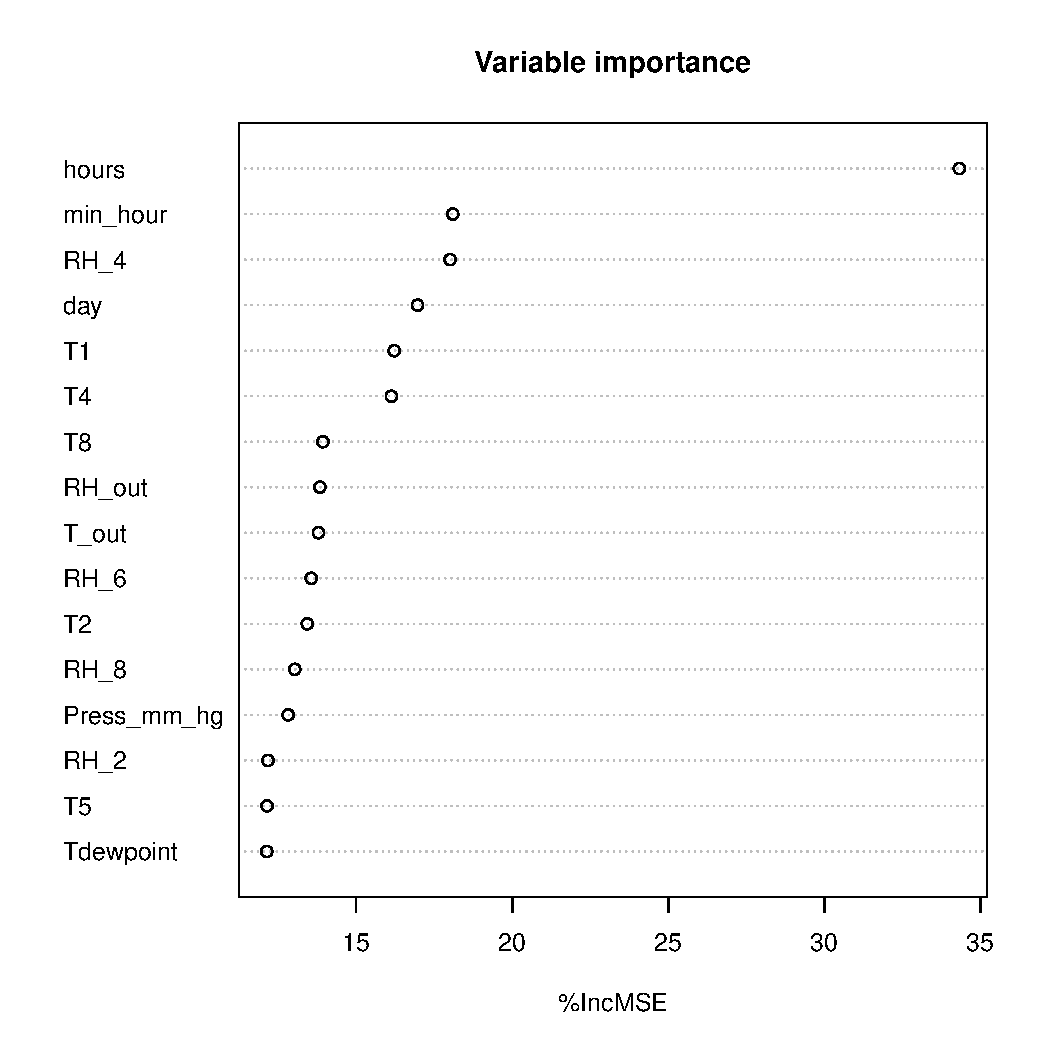
\includegraphics[page=1,
%%				width=0.8\linewidth,
%%				origin=c	
%%		]{../Rplots.pdf}
%%    }}%
%%    %\caption{TODO caption}%
%%    \label{FIG_1}%
%%\end{figure}
%
%\endgroup



\begingroup
\let\clearpage\relax
\chapter{Selekcja atrybutów}\label{chap:selekcja}

%TODO zajebane z elka.mine
Aby zapobiec nadmiernemu dopasowaniu, stosuje się selekcję atrybutów, która wybiera kilka najważniejszych atrybutów do późniejszego stworzenia modeli. Po zastosowaniu selekcji, modele oparte o ograniczoną liczbę atrybutów zwykle są lepsze od opartych o wszystkie atrybuty. Istnieje wiele metod selekcji atrybutów; w ramach projektu zostało sprawdzone kilka metod (w nawiasach umieszczono opcję type funkcji \textit{feature\_selection}):
\begin{itemize}
	\item[$\bullet$] prosty filtr statystyczny (\textit{,,simple''}) - pomiędzy każdym z atrybutów a celem regresji stosuje się miarę statystyczną, która określa zależność celu od danego atrybutu (dalej ,,miara zależności''). Następnie wybiera się kilka atrybutów o największej ,,mierze zależności''. W ramach regresji pomiędzy atrybutami ciągłymi zastosowano współczynnik korelacji (Pearsona);
	\item[$\bullet$] bazująca na drzewach losowych (\textit{,,rf''}) - w tym celu wykorzystano pakiet randomForest i jego wbudowaną opcję zwracają parametr IMPORTANCE (bazujący na mierze MSE), o możliwości konfiguracji ilości drzew;
	\item[$\bullet$] metoda RRELIEF (\textit{,,relief''}) - wersja algorytmu RELIEF do zastosowań w zadaniu regresji. Algorytm RELIEF, początkowo zaprojektowany dla zadania klasyfikacji binarnej, polega na losowym wybraniu obserwacji (jednego rekordu klasy+atrybuty). Następnie wyszukuje się \textit{k} najbardziej podobnych obserwacji tej samej klasy, oraz \textit{k} klasy przeciwnej. Dla każdego atrybutu oblicza się wagę istotności. Po wykonaniu \textit{trees\_num} operacji, wykonuje się średnią wag istotności. Atrybuty segreguje się według wag istotności. W zadaniu regresji stosuje się inne funkcje obliczające wagę np. funkcję rozkładu.
	%\item[$\bullet$] metoda "wrapper" (\textit{,,wrapper''})- podejście zakładające, że nie istnieje jedyny najlepszy podzbiór atrybutów niezależny od zastosowanego modelu. W tym celu wybrano algorytm \textit{rpart} do wyboru najistotniejszych atrybutów.
\end{itemize}
	
\par
W ramach projektu stosuje się następujące podejście: dla każdej wymienionej metody wykonuje się selekcję połowy atrybutów (\textit{part=0.5}) atrybutów, następnie wyznaczoną formułę aplikuje się do stworzenia modelu \textit{rpart()}, i procedurze oceny (10-krotnej walidacji krzyżowej \textit{model\_eval()}). Następnie największy współczynnik korelacji Pearsona wyznacza najlepszą metodę selekcji atrybutów oraz formułę do stworzenia modelu.

%TODO zajebane z twojego readme z gita
%Najprostszym, zadowalającym rozwiązaniem jest zastosowanie pakietu randomForest w celu wyznaczenia predykcyjnej przydatności atrybutów, a następnie wybór (może w kilku wariantach) pewnej liczby najlepszych atrybutów (np. najlepsze 25\%, 50\% itp.). W tym przypadku zalecałbym użycie miary "mean decrease accuracy", co wymaga użycia w wywołaniu funkcji randomForest argumentu importance=TRUE, zaś w wywołaniu funkcji importance lub varImpPlot argumentu type=1. Inne bardziej zautomatyzowane podejścia można znaleźć w kilku pakietach wymienionych tutaj: {\url{https://github.com/FrancisArgnR/R-FeatureSelection-Packages}}

\section{Wyniki selekcji atrybutów}

Na Rys. .... przedstawiono wyniki każdej z selekcji. W Tabeli \ref{table:wynikiSelekcji} przedstawiono porównanie wyników każdej z selekcji. Wynika z tego, że atrybuty wyznaczone metodą ..... pozwalają na najlepsze tłumaczenie modelu. Dla porównania przedstawiono też wynik walidacji krzyżowej dla modelu opartego o wszystkie atrybuty. Wynika 

\begin{table}[!h]  \centering
\caption{Wyniki selekcji atrybutów - współczynniki korelacji}
\begin{tabular} { c  c  c  c  c } \hline \hline
    \textbf{Parametr} & \textbf{\textit{randomForest}} & \textbf{\textit{simple}} & \textbf{\textit{RELIEF}} & \textbf{bez selekcji}  \\ \hline
    Appliances & 0,764 & 0,798 & 0,766 & 0,779 \\
    lights & 0,764 & 0,798 & 0,766 & 0,779 \\
    \hline \hline
    
\end{tabular}
\label{table:wynikiSelekcji}
\end{table}

\endgroup

\begingroup
\let\clearpage\relax
\chapter{Konstrukcja i ocena modeli}

\section{Metody konstrukcji modeli}
Pojedyncze modele drzew regresji zazwyczaj cierpią z powodu wysokiej wariancji -- jedną z metod jej redukcji jest tzw. Bagging (\textbf{B}ootstrap \textbf{agg}regat\textbf{ing}). 
Metoda ta polega na łączeniu i uśrednianiu wielu modeli drzew, co  zmniejsza wariancję i redukuje zbytnie dopasowanie.
%TODO dokładniejszy opis działania bo wydaje się mało
%Create m bootstrap samples from the training data. Bootstrapped samples allow us to create many slightly different data sets but with the same distribution as the overall training set.
%For each bootstrap sample train a single, unpruned regression tree.
%Average individual predictions from each tree to create an overall average predicted value.

Bagging może zostać zrealizowany za pomocą pakietu
\textit{ipred} 
lub
\textit{caret}. 
\textit{Ipred} jest z reguły prostszy w realizacji, jednakże stosowanie \textit{caret} niesie za sobą kilka zalet.
Znacznie prościej jest weryfikować krzyżowo wyniki -- pomimo możliwości wykorzystania błędu OOB (Out-of-Bag) w \textit{ipred}, weryfikacja krzyżowa daje dużo lepsze zrozumienie spodziewanego błędu. 
Dodatkowo możliwy jest dostęp do zmiennej odpowiedniości w wygenerowanych drzewach.
%TODO tłumaczenie potwierdź pls: We can assess variable importance across the bagged trees

%TODO który w końcu wybraliśmy
%TODO to co jest niżej jest zajebane z elka.mine, trzeba zmienić
Do konstrukcji modeli klasyfikacji został wykorzystany pakiet rpart budujacy drzewo klasyfikacji oraz pakiet
e1071, który umozliwia waidacje skrosna oraz automatyczny dobór parametrów w celu zmninimalizowania
błedu.

\section{Budowa modelu klasyfikacji z pakietu ipred}
%TODO pakiety R i parametry ~notatka z poprzedniego sprawka
TODO - pakiety R, parametry (np kryteria stopu, etc)

\section{Miary jakości}\label{sect:ocenamodeli}
Dla zbudowanych modeli oblicza się następujące miary jakości:
\begin{enumerate}
\item
CC - współczynnik korelacji liniowej Pearsona\\
\begin{gather*}
	CC =\frac{cov(P,A)}{var(P) \cdot var(A)}
\end{gather*}
\item
MSE - błąd średniokwadratowy
\begin{gather*}
	MSE = \frac{(p_1-a_1)^2+...+(p_n-a_n)^2}{n}
\end{gather*}
\item
RMSE - pierwiastek z błędu średniokwadratowego
\begin{gather*}
	RMSE = \sqrt{\frac{(p_1-a_1)^2+...+(p_n-a_n)^2}{n}}
\end{gather*}
\item
MAE - średni błąd względny
\begin{gather*}
	MAE = \frac{|p_1-a_1|+...+|p_n-a_n|}{n}
\end{gather*}
\item
RSE - względny błąd kwadratowy
\begin{gather*}
	RSE = \frac{(p_1-a_1)^2+...+(p_n-a_n)^2}{(a_1-\overline{a})^2+...+(a_n-\overline{a})^2}
\end{gather*}
\item
RRSE - pierwiastek ze względnego błędu kwadratowego
\begin{gather*}
	RRSE = \sqrt{\frac{(p_1-a_1)^2+...+(p_n-a_n)^2}{(a_1-\overline{a})^2+...+(a_n-\overline{a})^2}}
\end{gather*}
\item
RAE - błąd względny
\begin{gather*}
	RAE = \frac{|p_1-a_1|+...+|p_n-a_n|}{|a_1-\overline{a}|+...+|a_n-\overline{a}|}
\end{gather*}
\end{enumerate}
TODO tutaj ładnie się wpasuje co po kolei w kodzie poszło

\section{Procedury oceny}
Aby móc ocenić model pod względem przydatności zastosowano metodę k-krotnej walidacji krzyżowej. Kod zawarto w funkcji \textit{model\_eval()}, która stanowi . Zbiór testowy jest dzielony losowo na k podzbiorów równej wielkości. W kolejnych iteracjach każdy ze zbiorów jest traktowany jako zbiór testowy, podczas gdy na reszcie danych buduje się model. Następnie modele są uśredniane i następuje predykcja. Po predykcji modelu na zbiorze testowym wyznacza się miary jakości opisane w \ref{sect:ocenamodeli}.      


\endgroup




\begingroup
\let\clearpage\relax
\chapter{Wnioski}

TODO\\

\endgroup


%%%%%%%%%%%%%%%%%%%%%%%%%%%%%%%%%%%%%%%%%%%%%%%%%%%%%%%%%%%%%   
% 		Załączniki z kodem
%%%%%%%%%%%%%%%%%%%%%%%%%%%%%%%%%%%%%%%%%%%%%%%%%%%%%%%%%%%%%

%TODO nie wiem czy to potrzebne, ale daje objętość
%
\end{document}
